% 
% Learnings from scaling ironic at Yahoo.
%
% Copyright (C) 2017 Yahoo Inc.
%
% E-mail: saga@yahoo-inc.com
% Web: http://zer0c00l.in/
% Author; Arun S A G



\documentclass[aspectratio=169,11pt,hyperref={colorlinks=true}]{beamer}
\usetheme{boxes}
\usepackage{tikz}
\usetikzlibrary{arrows,shapes}
\setbeamertemplate{navigation symbols}{}
\definecolor{openstack}{RGB}{149,0,4}
\setbeamercolor{titlelike}{fg=openstack}
\setbeamercolor{structure}{fg=openstack}
\hypersetup{colorlinks,urlcolor=openstack}
\setbeamertemplate{footline}[frame number]
\usepackage{helvet}
\usepackage{graphicx}
\usepackage{color}
\usepackage{hyperref}
\usepackage{amsthm}
\usepackage{amsmath}
\usepackage[T1]{fontenc}
\usepackage{listings}
\newcommand\RBox[1]{%
  \tikz\node[draw,rounded corners,align=center,] {#1};%
}

\definecolor{mygreen}{rgb}{0,0.6,0}
\definecolor{mygray}{rgb}{0.5,0.5,0.5}
\definecolor{mymauve}{rgb}{0.58,0,0.82}

\lstset{%
  backgroundcolor=\color{white},   % choose the background color; you must add \usepackage{color} or \usepackage{xcolor}
  breakatwhitespace=false,         % sets if automatic breaks should only happen at whitespace
  breaklines=true,                 % sets automatic line breaking
  captionpos=b,                    % sets the caption-position to bottom
  commentstyle=\color{openstack},  % comment style
  extendedchars=true,              % lets you use non-ASCII characters; for 8-bits encodings only, does not work with UTF-8
  keepspaces=true,                 % keeps spaces in text, useful for keeping indentation of code (possibly needs columns=flexible)
  keywordstyle=\color{blue},       % keyword style
%  otherkeywords={*,...},           % if you want to add more keywords to the set
  numbersep=5pt,                   % how far the line-numbers are from the code
  numberstyle=\tiny\color{mygray}, % the style that is used for the line-numbers
  rulecolor=\color{black},         % if not set, the frame-color may be changed on line-breaks within not-black text (e.g. comments (green here))
  showspaces=false,                % show spaces everywhere adding particular underscores; it overrides 'showstringspaces'
  showstringspaces=false,          % underline spaces within strings only
  showtabs=false,                  % show tabs within strings adding particular underscores
  stringstyle=\color{openstack},   % string literal style
}

\setbeamerfont{caption}{series=\normalfont,size=\fontsize{6}{8}}
\setbeamertemplate{caption}{\raggedright\insertcaption\par}

\setlength{\abovecaptionskip}{0pt}
\setlength{\floatsep}{0pt}
\newcommand\Fontvi{\fontsize{6}{7.2}\selectfont}


\logo{
\includegraphics[scale=0.1]{logos/OpenStack_Logo_Horizontal.eps}}
\author[Arun S A G ]{%
    \texorpdfstring{%
        \centering
        Arun S A G\\
        \href{mailto:saga@yahoo-inc.com}{saga@yahoo-inc.com}\\
        \texttt{zer0c00l on freenode}
    }
    {Arun S A G}
}
\date{May 08, 2017}
\institute{\href{https://about.yahoo.com/}{Yahoo Inc}}

\title[Learnings from scaling Ironic at Yahoo \hspace{2em}\insertframenumber/\inserttotalframenumber]{Learnings from scaling Ironic at Yahoo}

\begin{document}

{%
\setbeamertemplate{background canvas}{
\includegraphics[width=\paperwidth,height=\paperheight]{logos/background.png}}
\setbeamertemplate{footline}{}

% title page
\begin{frame}[noframenumbering]
    \setbeamercolor{titlelike}{fg=white}
    \setbeamercolor{structure}{fg=white}
    \setbeamercolor{normal text}{fg=white}
    \hypersetup{colorlinks,urlcolor=white}
    \setbeamercolor{author}{fg=white}
    \setbeamercolor{date}{fg=white}
    \setbeamercolor{background}{bg=openstack}
    \titlepage{}
    \centering
    \href{https://github.com/sagarun/presentations}{https://github.com/sagarun/presentations/}
\end{frame}
}

\newcommand{\medsize}[1]{\fontsize{15}{15}\selectfont #1}
\newcommand{\bigsize}[1]{\fontsize{35}{35}\selectfont #1}



%\AtBeginSection[]
%{
%  \begin{frame}
%    \frametitle{Table Of Contents}
%    \tableofcontents[currentsection]
%  \end{frame}
%}

%\AtBeginSubsection[]
%{
%   \begin{frame}
%       \frametitle{Table Of Contents}
%       \tableofcontents[currentsection,currentsubsection]
%   \end{frame}
%}

\AtBeginSection[]{
  \begin{frame}
  \vfill
  \centering
  \begin{beamercolorbox}[sep=8pt,center,shadow=true,rounded=true]{title}
    \usebeamerfont{title}\insertsectionhead\par%
  \end{beamercolorbox}
  \vfill
  \end{frame}
}



\section{Background and Architecture}

\begin{frame}
\frametitle{Cluster Architecture}
    \begin{center}
        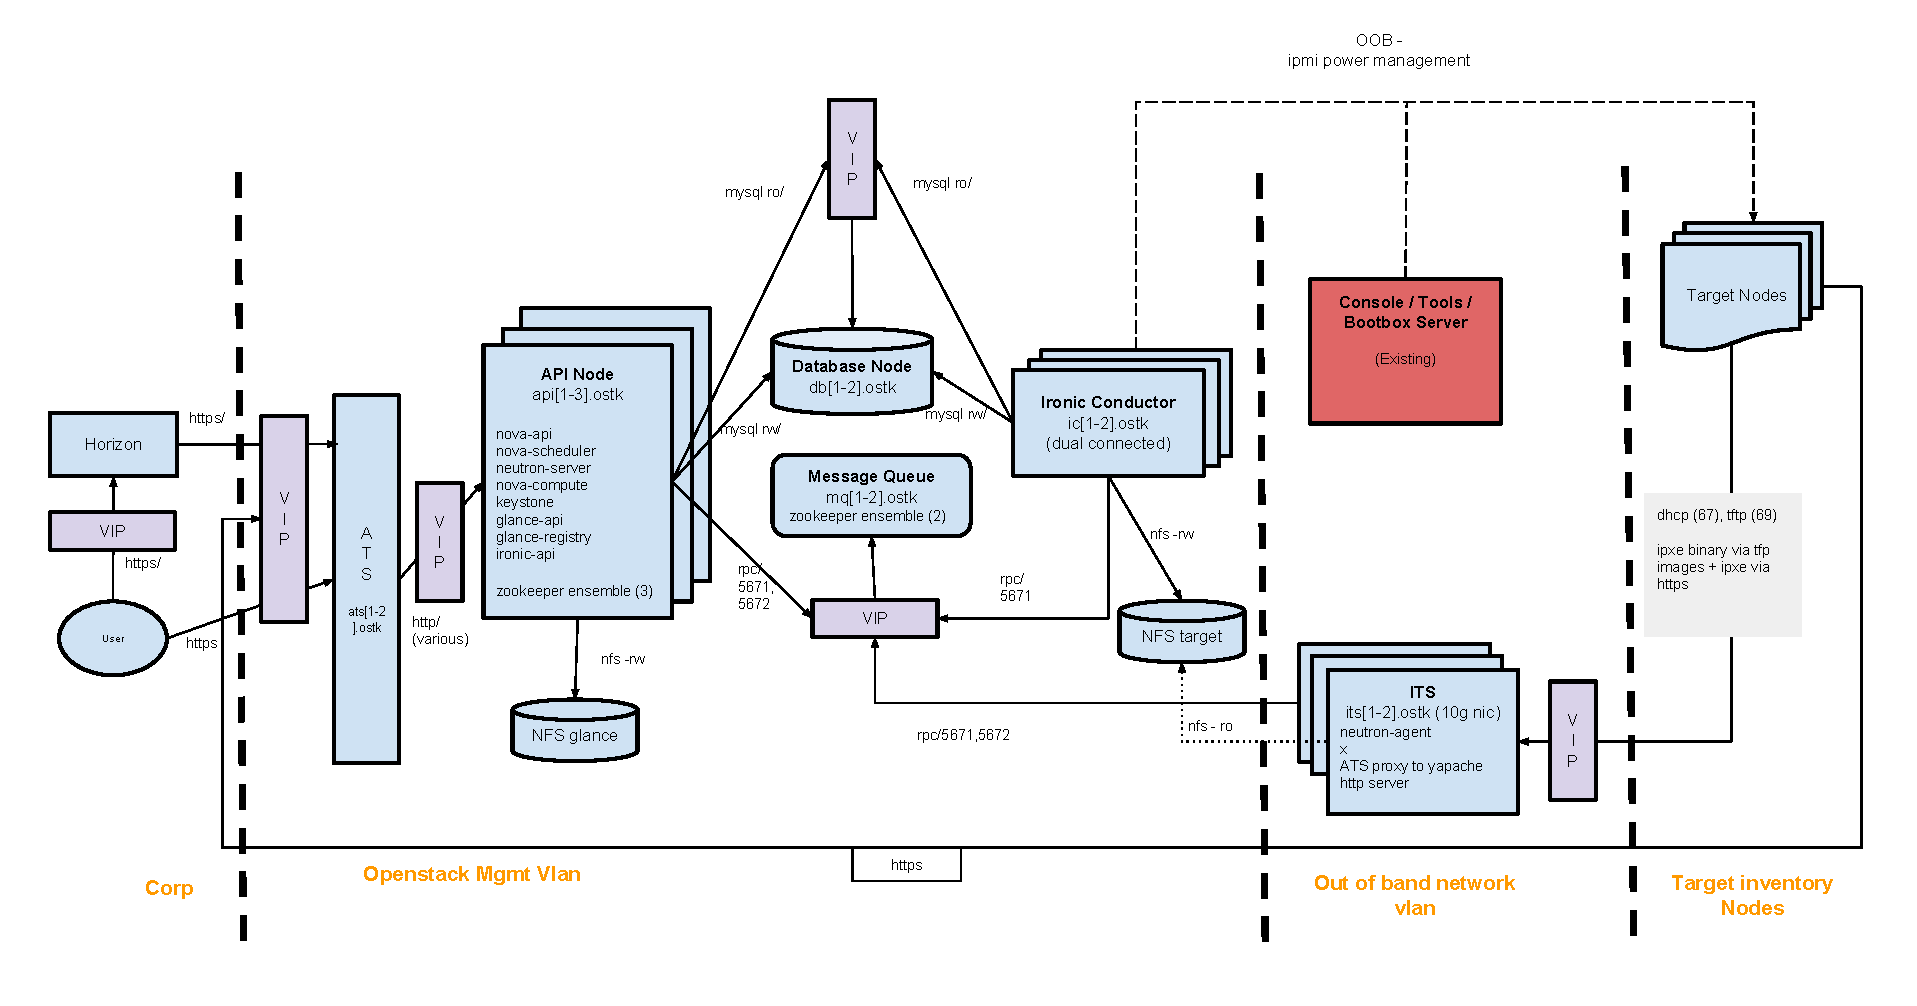
\includegraphics[scale=0.40]{logos/ironic_arch.pdf}
    \end{center}
\end{frame}


\begin{frame}
\frametitle{Migrating to Ironic}
    \begin{itemize}[<+-| alert@+>]
        \item Import nodes from old system into Ironic
        \item Create neutron port for the node
        \item If the node is already active in the old system, 'fake' boot it with fake\_pxe driver
        \item Once everything is successful, switch to pxe\_ipmitool driver
    \end{itemize}
\end{frame}

\section{Ironic}

\begin{frame}
\frametitle{Ironic Setup}
    \begin{itemize}[<+-| alert@+>]
        \item Ironic API runs behind Apache Server
        \item Ironic Conductors(2)
    \end{itemize}
\end{frame}

\begin{frame}
\frametitle{}
    \begin{center}
        
\includegraphics[scale=0.75]{logos/wrong2.jpg}
    \end{center}
\end{frame}

\begin{frame}
\frametitle{}
    \begin{center}
        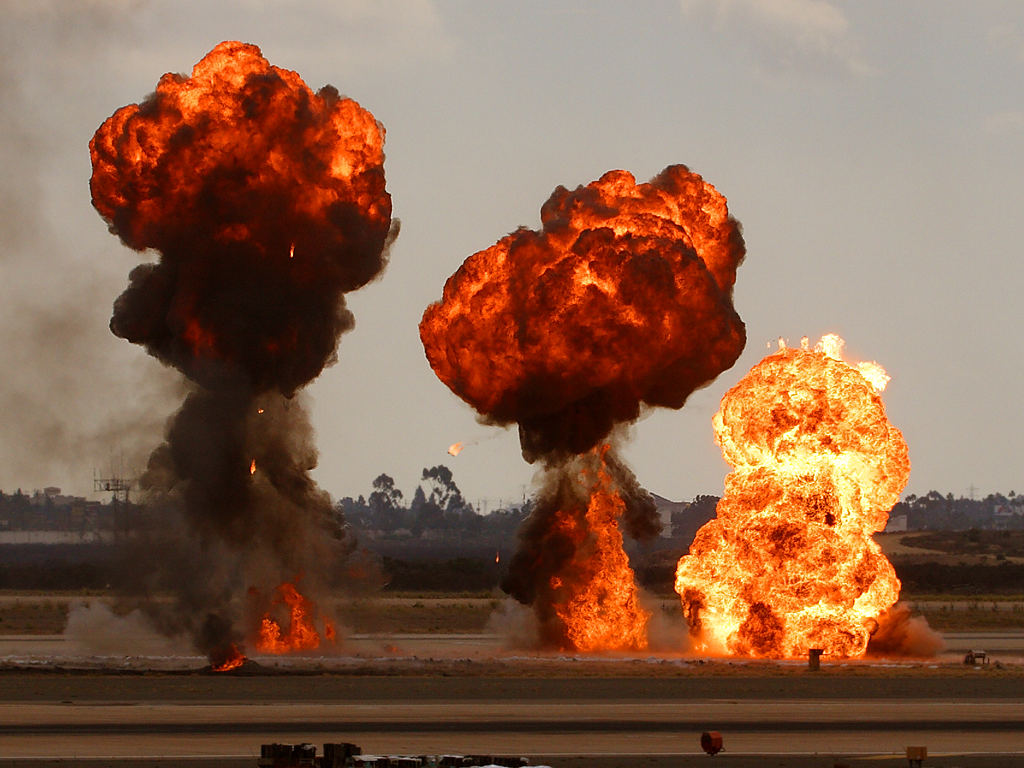
\includegraphics[scale=0.40]{logos/exp.jpg}
    \end{center}
\end{frame}



\begin{frame}
    \frametitle{What could possibly go wrong?}
    \begin{itemize}[<+-| alert@+>]
        \item Ironic Boots started to fail
        \item Ironic-conductor was using lot of CPU
        \item Ironic API calls took too long
    \end{itemize}
\end{frame}

\begin{frame}
    \frametitle{Solutions}
    \begin{itemize}[<+-| alert@+>]
        \item Sync\_Power\_State periodic task
        \item Increase the number of Ironic Conductors
        \item Run multiple conductors on the same host
    \end{itemize}
\end{frame}


\section{Neutron}
\begin{frame}
    \frametitle{Neutron setup}
    \begin{itemize}[<+-| alert@+>]
        \item All 3 API servers run neutron-server
        \item 24 API/RPC workers
        \item 4 neutron dhcp agents
        \item All networks/subnets are managed by all 4 agents (HA)
        \item ISC DHCPD driver instead of dnsmasq
    \end{itemize}
\end{frame}

\section{What is sync state?}
\begin{frame}
    \frametitle{A tale of two drivers}
    \begin{itemize}[<+-| alert@+>]
        \item OMShell driver
        \item Pypureomapi driver
    \end{itemize}
\end{frame}

\begin{frame}[fragile]
    \frametitle{OMShell}
    \Fontvi
\begin{verbatim}
-bash-4.1$ omshell
> server 127.0.0.1
> port 7911
> key keyname secret
> connect
obj: <null>
> new host
obj: host
> set hardware-address = 00:1c:1a:1d:10:54  
obj: host
hardware-address = 00:1c:1a:1d:10:54
> open
obj: host
hardware-address = 00:1c:1a:1d:10:54
ip-address = 0a:d7:a6:b1
name = "hostname.yahoo.com-0"
hardware-type = 00:00:00:01
>remove
    \end{verbatim}
\end{frame}

\begin{frame}
    \frametitle{Sync State with OMShell}
     \begin{center}
         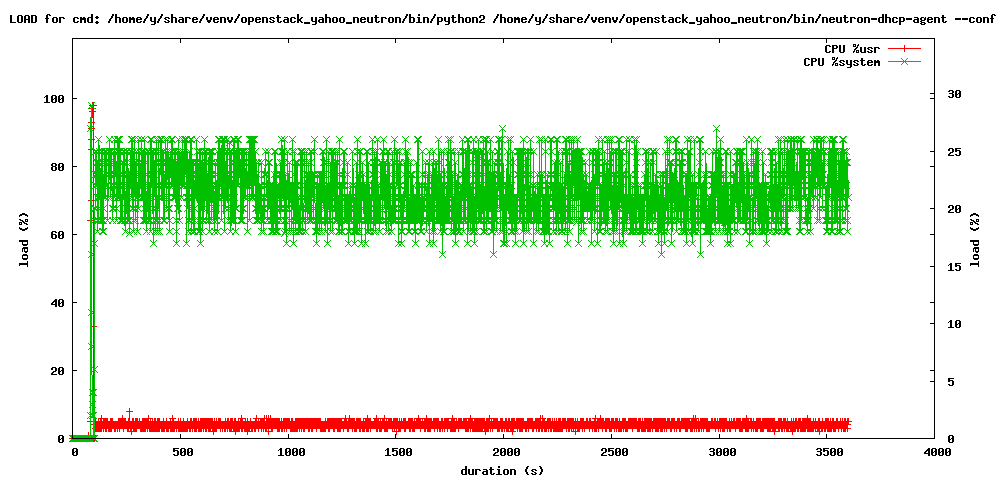
\includegraphics[scale=0.35]{logos/omshell.png}
    \end{center}
\end{frame}


\begin{frame}
    \frametitle{Sync State with PypureOMAPI}
     \begin{center}
         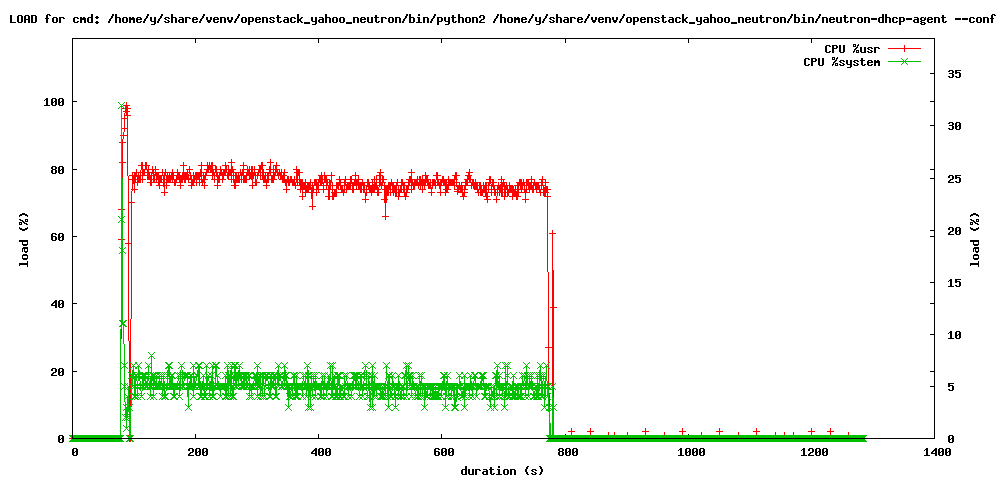
\includegraphics[scale=0.35]{logos/pypureomapi.png}
    \end{center}
\end{frame}

\begin{frame}
    \frametitle{Where do we go from here?}
    \begin{itemize}[<+-| alert@+>]
        \item ISC DHCPD restarts are not ideal
        \item VIP thinks dhcpd is down whenever it restarts
        \item Move to Kea DHCP Server
    \end{itemize}
\end{frame}

\section{Density Test}
\begin{frame}
    \frametitle{When did things started to break?}
    \begin{itemize}
        \item At ~24500 nodes, API servers started swapping
    \end{itemize}
\end{frame}

\begin{frame}
    \frametitle{Swap and memory usage on API nodes}
    \begin{columns}[t]
    \column{.5\textwidth}
    \centering
        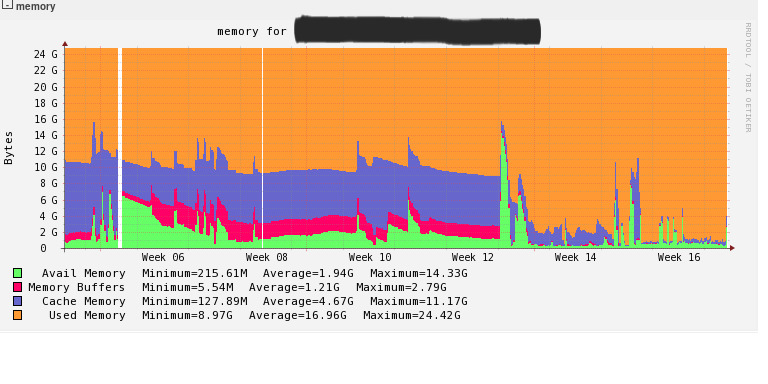
\includegraphics[scale=0.30]{logos/mem_api.png}\ 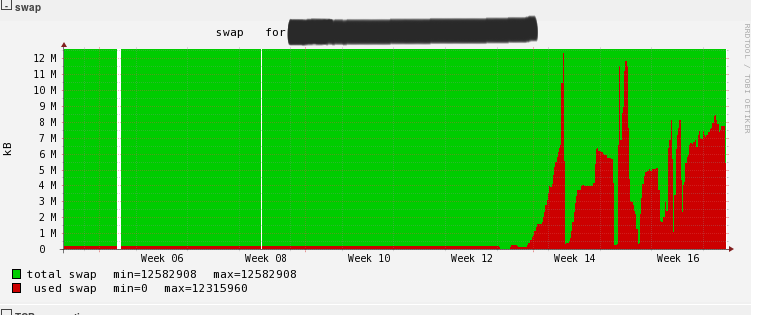
\includegraphics[scale=0.30]{logos/swap_api.png}
    \end{columns}
\end{frame}

\begin{frame}
    \frametitle{Memory usage}
    \begin{itemize}[<+-| alert@+>]
        \item Neutron the biggest user of memory: ~1.4 GB per process
        \item Subnets: 2500 Ports: 43000
        \item Easy fix: Reduce  number of api\_workers and rpc\_workers
        \item Long Term Fix: Investigate memory usage, isolate neutron
    \end{itemize}
\end{frame}

\section{Learnings}
\begin{frame}
    \frametitle{Learnings}
    \begin{itemize}[<+-| alert@+>]
        \item Do a *density* and *scale* testing before taking on production
        \item Avoid spawning processes, try and use native python libraries whenever possible
        \item Pay attention to periodic tasks
        \item Be prepared to scale horizontally
        \item Pay attention to number of workers,conductors,rpc\_workers
        \item Don't forget to have fun :)
    \end{itemize}
\end{frame}


\section{Questions}

\begin{frame}
    \frametitle{References}
    \begin{itemize}
        \item Layout and background: https://github.com/mtreinish/openstack-health-presentation
        \item Picture from TV show: http://www.imdb.com/title/tt4338930/
        \item Picture of explotion: https://en.wikipedia.org/wiki/Explosion
    \end{itemize}
\end{frame}
\end{document}
